%%This is a very basic article template.
%%There is just one section and two subsections.
\documentclass[11pt, a4paper, reqno, twoside]{scrartcl}

\usepackage[a4paper, hmargin={1in, 1in}, vmargin={1in,
  1in},headsep=10mm,headheight=5mm,footskip=30pt]{geometry}
 \usepackage{graphicx}
\usepackage{epsfig}
\usepackage{epstopdf}
\graphicspath{ {./images/} }

\usepackage{ amsmath, amssymb,amsthm}
\usepackage{hyperref}
\usepackage{bm,color}
\usepackage{verbatim}
\usepackage{wrapfig}
\usepackage{caption}
\usepackage{subcaption}
\usepackage{tikz}
\usepackage{tkz-euclide}
\usetkzobj{all}
\usepackage[boxruled,commentsnumbered]{algorithm2e}
\usepackage{booktabs}

\usepackage{fancyhdr}
  \renewcommand{\baselinestretch}{0.97} %this factor controls the space between lines
  \fancyhead[]{}
  \renewcommand{\headrulewidth}{0pt}

% the only way to get two column algorithms seems to be to use a hack on top of the algorithm2e package
\usepackage{multicol}
%\usepackage[ruled,commentsnumbered]{algorithm2e}

\newenvironment{algo}{%
  \renewenvironment{algocf}[1][h]{}{}% pass over the floating stuff
  \algorithm
}{%z
  \endalgorithm
}

\definecolor{darkgreen}{rgb}{0,.4,.2}
\definecolor{darkblue}{rgb}{.1,.2,.6}
\definecolor{brightblue}{rgb}{0,0.6,0.8}
\hypersetup{
  colorlinks=true,
  linkcolor=darkblue,
  citecolor=darkgreen,
  filecolor=darkblue,
  urlcolor=darkblue
}
\usepackage{pifont}% http://ctan.org/pkg/pifont
\newcommand{\cmark}{\ding{51}}%
\newcommand{\xmark}{\ding{55}}%

\addtokomafont{caption}{\small}
\addtokomafont{captionlabel}{\sffamily\bfseries}

\newtheoremstyle{style}
 {\topsep}              % Space above
 {\topsep}              % Space below
 {\itshape}              % Body font: original {\normalfont}
 {}                         % Indent amount (empty = no indent,%\parindent = paraindent)
 {\sffamily\bfseries}  % Thm head font original
 {.}	                     % Punctuation after thm head
 { }                         % Space after thm head (\newline = linebreak)
 {}                          % Thm head spec
\theoremstyle{style}

%%%%%%%%%%%%%%%%%%%%%%%%%%%%%%%%%%%%%%%%%%%
%%% Environments, Definitions, Commands %%%
%%%%%%%%%%%%%%%%%%%%%%%%%%%%%%%%%%%%%%%%%%%

\newtheorem{definition}{Definition}
\newtheorem{theorem}{Theorem}
\newtheorem{proposition}[definition]{Proposition}
\newtheorem{lemma}{Lemma}
\newtheorem{corollary}[definition]{Corollary}
\newtheorem{observation}[definition]{Observation}
\newtheorem{conjecture}[definition]{Conjecture}
\newtheorem{remark}[definition]{Remark}
\newtheorem{problem}{Problem}
\newtheorem{claim}{Claim}
\newtheorem{open}{Open Problem}
\newtheorem*{example}{Example}

% the * at the end of operator seems to have the effect that the command will be properly have its sub/superstripts vertically below/above it, like \sum for example, this only applies if you are in \displaystyle
\DeclareMathOperator{\st}{\textrm{s.t.}}
\DeclareMathOperator*{\conv}{conv}
\DeclareMathOperator{\diam}{diam}
\DeclareMathOperator*{\E}{\rm E}
\DeclareMathOperator*{\argmin}{\arg\min}
\DeclareMathOperator*{\argmax}{\arg\max}
\DeclareMathOperator{\lmax}{\lambda_{\max}}
\DeclareMathOperator{\lmin}{\lambda_{\min}}
\DeclareMathOperator*{\supp}{supp}
\DeclareMathOperator*{\diag}{diag}
\DeclareMathOperator*{\sign}{sign}
\DeclareMathOperator*{\tr}{Tr}
\DeclareMathOperator*{\rk}{Rk}
\DeclareMathOperator*{\card}{card}
\DeclareMathOperator*{\nnz}{nnz}
\DeclareMathOperator*{\relint}{\mathop{relint}}

%norms
\providecommand{\abs}[1]{\left\lvert#1\right\rvert}
\providecommand{\norm}[1]{\left\lVert#1\right\rVert}

\newcommand{\ball}{\mathcal{B}}
\newcommand{\sphere}{\mathcal{S}}

\newcommand{\bigO}{O}
\newcommand{\R}{\mathbb{R}}
\newcommand{\X}{\mathcal{X}}
\newcommand{\Sym}{\mathcal{S}}
\newcommand{\Supt}{\Sym_{(t)}}
\newcommand{\Suptc}{\bar{\Sym}_{(t)}}

\newcommand{\appcof}{v}
\newcommand{\domain}{\mathcal{D}}

\newcommand{\points}{\mathcal{A}}
\newcommand{\stepsize}{\gamma}
\newcommand{\Cf}{C_{\hspace{-0.08em}f}}
\newcommand{\x}{\bm{x}}
\newcommand{\y}{\bm{y}}
\newcommand{\z}{\bm{z}}
\newcommand{\s}{\bm{s}}
\newcommand{\shat}{\bm{\hat{s}}}
\newcommand{\bv}{\bm{b}}
\newcommand{\dv}{\bm{d}}
\newcommand{\qv}{\bm{q}}
\newcommand{\uv}{\bm{u}}
\newcommand{\av}{\bm{v}}
\newcommand{\vv}{\bm{v}}
\newcommand{\wv}{\bm{w}}
\newcommand{\xv}{\bm{x}}
\newcommand{\row}{\text{row}}
\newcommand{\col}{\text{col}}
\newcommand{\lft}{\text{left}}
\newcommand{\rgt}{\text{right}}
\newcommand{\dualp}{\bm{\alpha}}
%
\newcommand{\signVec}{\mathbf{s}}
\newcommand{\N}{\mathbb{N}}
\newcommand{\F}{\mathbb{F}}
\newcommand{\M}{\mathbb{M}}
\newcommand{\id}{\mathbf{I}} % big i for identity
\newcommand{\ind}{\mathbf{1}} % indicator vectors
\newcommand{\0}{\mathbf{0}} % the origin
\newcommand{\unit}{\mathbf{e}} % unit basis vectors
\newcommand{\one}{\mathbf{1}} % all one vector
\newcommand{\zero}{\mathbf{0}}
\newcommand\SetOf[2]{\left\{#1\vphantom{#2}\right.\left|\vphantom{#1}\,#2\right\}}
\newcommand{\ignore}[1]{}%{\textbf{***begin ignore***}\\#1\textbf{***end ignore***}}


\newcommand{\todo}[1]{\marginpar[\hspace*{4.5em}\textbf{TODO}\hspace*{-4.5em}]{\textbf{TODO}}\textbf{TODO:} #1}
\newcommand{\idea}[1]{\marginpar[\hspace*{4.5em}\textbf{IDEA}\hspace*{-4.5em}]{\textbf{IDEA}}\textbf{IDEA:}
#1}
\newcommand{\note}[1]{\marginpar{#1}}





\begin{document}
\pagestyle{fancy}



%%%%%%%%%%%%%%%%%%%%%%%%%%%%%%%%
\title{Learning with Adaptive Sample Sizes}

%\author{\\ Author Name\\
%{\small \href{mailto:author@ethz.ch}{author@ethz.ch}}}
\date{} 

\maketitle
\section{Updates}
\begin{itemize}
  \item Section 4: Loss sub-optimality discussion
\end{itemize}

\section{SAGA} 
For a $\mu$-strongly convex loss, with Lipschitz constant $L$, we have the
following learning rate and convergence rate: 
\begin{eqnarray}
& \gamma_m & = \min\{ \frac{1}{m}, \frac{\mu}{L} \} \nonumber\\ 
& \E \bigg[ \| \wv^s -\wv^*_m \|^2 \bigg] & \leq
(1-\gamma_m)^s\bigg(\underbrace{\| \wv^0 -\wv^*_m \|^2 + m\gamma_m [R_m(\wv^0)
- \langle R_m^{'}(\wv^*_m),\wv^0 - \wv^* \rangle - R_m(w^*_m)
]}_{C_{\gamma_m}(\wv^0,\wv^*_m)} \bigg)
\label{eqn:saga_convergence}
\end{eqnarray}
Please note that the Lipschitz constant L, for both of logistic loss and the
regression case, is bounded by $L \leq \max_i \|\xv_i\|$. Let's rewrite the loss
function for logistic regression: 
\begin{equation}
	f_i(\wv) = \log(1+ \exp(-y_i \langle \wv, \xv_i \rangle)) + \lambda/2
	\|\wv\|^2_2
	\nonumber
\end{equation}
Then the Hessian matrix of this loss would be: 
\begin{equation}
	H_f(\wv) = \frac{x_i x_i^T \exp(-y_i \langle \wv, \xv_i \rangle)}{(1+\exp(-y_i
	\langle \wv, \xv_i \rangle))^2} + \lambda I \nonumber
\end{equation}
We know that $x_i x_i^T$ is a rank one matrix and it never can be a
semi-positive definite matrix. Consequently, the $\mu = \lambda$ always holds.
Finally, we have the following convergence rate for $m$ samples: 
\begin{equation}
	\gamma_m  = \min \{ \frac{1}{m}, \frac{\lambda}{L} \}
\end{equation}
Lets compute the number of passes $k$ that saga needs to hit the $r_n = \| \wv^*
- \wv^*_n \|^2 = O(\frac{1}{\sqrt{n}})$. 
\begin{equation}
	(1-1/n)^{k n} (\| \wv^{k n} - \wv^*_n \|^2) \leq exp(-k) \leq
	\frac{1}{\sqrt{n}}
\end{equation}
So, we need $O(\ln(n)-1)$ passes over data. In our setting $n= 10^5$, so we need
$11.5$ passes over data. We want to reduces this passes to just one pass over
the data. 
\section{Geometrical Discussion}
\subsection{Thomas's Geometric Set-up:}
In Thomas's geometrical trade-off, we have two options:
\begin{itemize}
  \item Iterate on $n$ samples: $w_n^+$ denotes the updated parameter after one
  iteration on objective achieved by $n$ samples. According to the
  convergence rate we have:
  \begin{equation} \label{eqn:onestepn}
  	\|\wv_n^+ - \wv_n^*\|^2 \leq (1-\mu \gamma_n) \|\wv_s - \wv_n^* \|^2 
  \end{equation}
  \item Iterate on $m$ samples: $w_m^+$ denotes the updated parameter after one
  step on objective obtained by $m$ samples. In this case we have: 
  \begin{equation}
  	\|\wv_m^+ - \wv_m^*\|^2 \leq (1-\mu \gamma_m) \|\wv_s - \wv_m^* \|^2
  	\nonumber
  \end{equation}
\end{itemize}
Clearly, we want to make the largest step towards $\wv_n^*$. To this end, we
need to check $\|\wv_m^+ - \wv_n^*\| \leq_{?} \|\wv_n^+ - \wv_n^*\|$ to choose
between two above options.
As the first step, we have to rewrite the convergence equation for $m$ samples
using the geometric structure shown in figure \ref{fig:geometric} and considering that
$\langle\wv_m^+-\wv_m^*,\wv_m^*-\wv_n^*\rangle = 0$
\begin{eqnarray}
  & \|\wv_m^+ - \wv_n^*\|^2 & = \|\wv_m^+ - \wv_m^*\|^2+\|\wv_m^* -
  \wv_n^*\|^2 \nonumber \\ 
  & & \leq_{\text{using \ref{eqn:onestepn}}} (1-\mu \gamma_m) \|\wv_s - \wv_m^*
  \|^2 +\|\wv_m^* - \wv_n^*\|^2 \nonumber
\end{eqnarray}
Secondly, we have to compute $\|\wv^s - \wv_n^*\|$ as well:
\begin{eqnarray}
& \|\wv^s - \wv_n^*\|^2 & = \|\wv^s -
\wv_m^*\|^2+\|\wv_m^* - \wv_n^*\|^2 \nonumber
\end{eqnarray} 
Thirdly, we can proceed computing $\|\wv_n^+ - \wv_n^*\|$: 
\begin{eqnarray}
	& \|\wv_n^+ - \wv_n^*\|^2 & \leq_{\text{using \ref{eqn:saga_convergence}}}
	(1-\mu \gamma_n) \|\wv_s - \wv_n^*\|^2  \nonumber\\ 
	& & \leq (1-\mu \gamma_n)\bigg(\|\wv^s -
\wv_m^*\|^2+\|\wv_m^* - \wv_n^*\|^2\bigg) \nonumber
\end{eqnarray}
Now, instead of investigation of $\|\wv_m^+ - \wv_n^*\| \leq_{?} \|\wv_n^+ -
\wv_n^*\|$ we check their upper bounds:
\todo{Checking the effect of upper bounds!}
\begin{equation}
	(1-\mu \gamma_m) \|\wv_s - \wv_m^* \|^2
  +\|\wv_m^* - \wv_n^*\|^2 \leq_{?} (1-\mu \gamma_n)\bigg(\|\wv^s -
\wv_m^*\|^2+\|\wv_m^* - \wv_n^*\|^2\bigg) \nonumber
\end{equation}
Now, we can bound the $ \|\wv_s - \wv_m^* \|$ easily using the convergence rate,
still we have to bound $\|\wv^s - \wv_m^*\|^2$. Before that, let's us just
simplify the above equality as follows: 
\begin{equation}
\frac{\gamma_n}{\gamma_m - \gamma_n} \leq_{?} \frac{\|\wv^s -
\wv_m^*\|^2}{\|\wv_m^* - \wv_n^* \|^2} \label{eqn:tradeoff}
\end{equation}
\textbf{Remark:} we can make the tradeoff for $k$ steps forward tradeoff. In the
new setting, we make decision for $k$ steps forwards instead of just one step
forward. Considering the new setting the critical formula can be written as: 
\begin{equation*}
	\frac{1- (1-\gamma_n)^k}{(1 -\gamma_n)^k - (1-\gamma_m)^k} \leq_{?}
	\frac{\|\wv^s - \wv_m^*\|^2}{\|\wv_m^* - \wv_n^* \|^2} 
\end{equation*}

\begin{figure}
	
	\begin{center}
		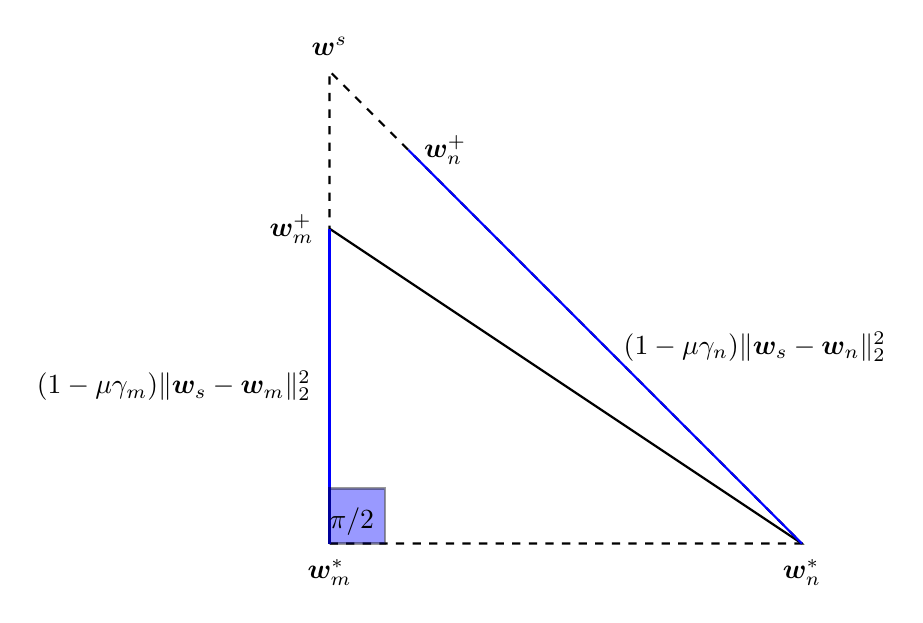
\begin{tikzpicture}[thick]
		\coordinate (O) at (0,0);%xm
		\coordinate (A) at (6,0);%xn
		\coordinate (B) at (0,6);%xs
		\coordinate (C) at (0,4);%xm+
		\coordinate (D) at (1,5);%xn+
		\draw [dashed] (O)--(A)--(B)--cycle;
		\draw (C)--(A);
		\draw [blue] (C)--(O);
		\draw [blue] (D)--(A);
		
		\tkzLabelSegment[left=3pt](C,O){\textit{$(1-\mu \gamma_m) \|\wv_s - \wv_m
		\|^2_2 $}} \tkzLabelSegment[right=3pt](D,A){\textit{$(1-\mu \gamma_n) \|\wv_s
		- \wv_n \|^2_2 $}} \tkzLabelSegment[below=2pt](O,O){\textit{$\wv_m^*$}}
		\tkzLabelSegment[below=2pt](A,A){\textit{$\wv_n^*$}}
		\tkzLabelSegment[above=2pt](B,B){\textit{$\wv^s$}}
		\tkzLabelSegment[left=2pt](C,C){\textit{$\wv^+_m$}}
		\tkzLabelSegment[right=2pt](D,D){\textit{$\wv^+_n$}}
		
		\tkzMarkRightAngle[fill=blue,size=0.7,opacity=.4](A,O,B)% square angle here
		\tkzLabelAngle[pos = 0.4](A,O,B){$\pi/2$}
		\end{tikzpicture}
	\end{center}
	\caption{Geometric Structure: we want to compare the length of $\|\wv_m^+ -
	\wv_n^* \|$ segment with segment $\|\wv_n^+ -\wv_n^* \|$}
  \label{fig:geometric}
\end{figure}
 \subsection{Generalization bound}
 Our notations are summarised in the following table. Indeed, our goal is
 to infer a function, still we assumed this function is a parametric map, from
 input vector $\xv$ to label $y$, and use the parameters instead of the function
 notation. Our notations are
 inspired by paper \cite{bousquet2004introduction}.
\begin{eqnarray}
    & \N = \{1,\ldots,n\} & \text{Training indices} \nonumber\\ 
    &  \Cf & \text{Domain of $\wv$ induced by function
    space} \nonumber\\
     & R_n(\wv) = \frac{1}{n} \sum_{i\in \N} \ell(f(\xv_i;\wv),y_i)&
    \text{ Empirical Risk on $\N$} \nonumber\\
    & R_{m}(\wv) = \frac{1}{m} \sum_{i \in \M} \ell(f(\xv_i;\wv),y_i)&
    \text{Empirical Risk on $\M\subset \N$}\nonumber\\ 
    & \wv_n^* = \argmin_{\wv \in \Cf} R_n(\wv) &\text{Empirical Risk Minimizer
    on $\N$}\nonumber\\
    & \wv_m^* = \argmin_{\wv \in \Cf} R_m(\wv) &\text{Empirical Risk Minimizer
    on $\M$}\nonumber\\ 
    & R(\wv) = E_{\xv,y\sim P}[\ell(f(\xv;\wv),y)]&\text{ Expected Risk}
    \nonumber\\
    & \wv^* = \argmin_{\wv\in \Cf} R(\wv) &\text{The true best estimator}
    \nonumber
\end{eqnarray}

 If the loss function $\ell$ is strongly convex respect to parameter
 vector $\wv$, then $R_n$, as non-negative sum of strongly convex functions, is
 strongly convex as well. This equips us to bound $\|\wv^* - \wv_n^*\| $
 using bound on $R_n(\wv^*) - R_n(\wv_n^*)$: 
 \begin{eqnarray}
 	R_n(\wv^*) - R_n(\wv_n^*) \geq \nabla R_n(\wv_n^*) (\wv^* - \wv_n^*)
 	+\frac{\mu}{2} \|\wv^* - \wv_n^* \|^2 \nonumber
 \end{eqnarray}
 Since the $w_n^*$ is the optimal parameter of empirical risk $R_n$, we can
 assume its gradient is zero i.e. $\nabla R_n(\wv_n^*) = 0$. Consequently, we
 can bound distance of parameters using the bound on risks. 
 \begin{equation}
 	\frac{2}{\mu}\bigg(R_n(\wv^*) - R_n(\wv_n^*)\bigg) \geq  \|\wv^* - \wv_n^*
 	\|^2 \label{eqn:strongconvexity}
 \end{equation}
 The Naive approach to deal with this bound is using the optimal parameter
 $\wv^*$ of expected risk to factorise this bound on two separated
 generalization bounds $G_m$ and $G_n$ as follows:
 \begin{eqnarray}
  & R_n(\wv^*) - R_n(\wv_n^*) & = \underbrace{R_n(\wv^*) - R(\wv^*)}_{G^*}
  \nonumber \\ 
  & & + \underbrace{R(\wv^*) - R_n(\wv_n^*)}_{G_n^*}  + \underbrace{R(\wv_n^*) -
  R_n(\wv_n^*)}_{G_n}\label{equ:generalization_inequality}
 \end{eqnarray}
 The basic theorems of statistical learning theory says that the following
 inequality holds with at least probability $1 - \delta$
 \begin{equation}
 	\wv \in C_f, R(\wv) \leq R_n(\wv) + 2 \sqrt{2 \frac{h \log \frac{2e
 	n}{h} + \log \frac{2}{\delta}}{n}} \nonumber
 \end{equation}
In addition, one can easly shows that \cite{bousquet2004introduction}: 
\begin{equation}
	R(\wv_n^*) -  R(\wv^*) \leq 2 \sup_{\wv \in C_f}[R(\wv) - R_n(\wv)] \nonumber
\end{equation}
Using two above inquality we can bound $G_n$, $G^*$, and $G_n^*$ at inequality
\ref{equ:generalization_inequality}; 
\begin{equation}
	R_n(\wv^*) - R_n(\wv_n^*) \leq 8 \sqrt{2 \frac{h \log \frac{2e
 	n}{h} + \log \frac{2}{\delta}}{n}}	\nonumber
\end{equation}
Above bound together with the strongly convex inequality
\ref{eqn:strongconvexity} yields us the following bound: 
\begin{equation}
	\| \wv_n^* - \wv^* \|^2 \leq \frac{16}{\mu}  \sqrt{2 \frac{h \log \frac{2e
 	n}{h} + \log \frac{2}{\delta}}{n}}	 \nonumber
\end{equation}
Now using this inequality we can bound distance between $\wv_n^*$ and $\wv_m^*$
with probability $1-\delta$:
\begin{eqnarray}
	& \| \wv_n^* - \wv_m^* \|^2 & \leq \| \wv_n^* - \wv^* \|^2  + \| \wv_m^* -
	\wv^* \|^2 \nonumber\\ 
	& & \leq \frac{16 \sqrt{2}}{\mu} \bigg[ \sqrt{\frac{h \log \frac{2e
 	n}{h} + \log \frac{2}{\delta}}{n}} +  \sqrt{ \frac{h \log \frac{2e
 	m}{h} + \log \frac{2}{\delta}}{m}} \bigg] \label{eqn:boundonoptimals}
\end{eqnarray}
\subsection{Geometrical tradeoff again} 
Now, let rewrite the geometrical tradeoff inequality \ref{eqn:tradeoff} using
the equation \ref{eqn:boundonoptimals} achieved by generalization discussion.
Here, we replace the upper bound for both of nominator $\|\wv^s -
\wv_m^*\|^2$, using the convergence rate, and denominator $\|\wv_m^* - \wv_n^*
\|^2$, using the result of generalization bound.
\begin{eqnarray}
& \frac{\gamma_n}{\gamma_m - \gamma_n} & \leq_{?} \frac{(1-\gamma_m)^s
C_{\gamma_m}(\wv^0,\wv^*_m)}{\frac{8}{\mu}
	 \sqrt{2\frac{h\log(\frac{2m}{h})+\log(\frac{2}{\delta}))}{m}}}
	 \label{equ:ratio_tradeoff_theory}
\end{eqnarray}
\textbf{Rough Analysis}: We skip all constants for simplicity.
\begin{eqnarray}
	& \frac{n^{-1}}{m^{-1} - n^{-1}} & \sim \frac{(1-1/m)^s}{\sqrt{h/m}}
	\nonumber\\
	& \frac{1}{n/m - 1} & \sim \frac{(1-1/m)^s}{\sqrt{h/m}}
	\nonumber\\
	& (1-1/m)^s & \sim \frac{\sqrt{h/m}}{n/m - 1} \nonumber \\ 
	& s \log(1-1/m) & \sim \frac{1}{2}\log h/m - \log(n/m-1) \nonumber \\ 
	& s & \sim \frac{\frac{1}{2}\log h/m - \log(n/m-1)}{\log(1-1/m)}\nonumber
\end{eqnarray}
The plot of the function $s$ for different values of $m$, when $n = 10000$, and
$h = 100$, is presented at figure \ref{fig:tradeoff_10000_100}. This
plot is very interesting because when the sample size $m$ is relatively small, then
number of iterations $s$, before switching to $n$ samples, is more than sample
size.
This contradicts to Leon Bottou's paper, where they claimed it  is always better
to do one pass over data using SGD. Nonetheless, their claims is regarding
the generalization bound and our results are on empirical risk convergence.
Except the negative part of the plot, the remaining parts seems reasonable. Indeed, for more samples
we needs more iterations and at some points when $m$ is very large, then it is
better switch to $n$ samples because two objectives $R_n$ and $R_m$ are close to
each other. The Figure \ref{fig:tradeoff_10000_1000} shows the plot for a larger
VC dimension $h = 1000$.
\subsection{Convergence Analysis of the Adaptive Sampling}
Let us rewrite the tradeoff
\label{eqn:tradeoff} for switching from $m$ to $2 m$: 

\begin{eqnarray}
 1 = \frac{\|\wv^s -
\wv_m^*\|^2}{\|\wv_m^* - \wv_{2m}^* \|^2}
\end{eqnarray} 
So, we go towards the $\wv_m^*$
as long as we are outside the statistical precision ball $\|\wv_m^* - \wv_{2m}^*
\|^2$; Then we switch to $2m$ samples. This trade-off should be treated
different at first step, middle steps, and the last step to propose a better
convergence rate.\\
\textbf{First Step:} Now, we compute the number of iteration, i.e. $s_1$, on
 $m$ samples before switching to $2m$.
 \begin{equation*}
	(1-1/m)^{s_1} \| \wv^0 - \wv_m^* \|^2 = \| \wv_m^* - \wv^*_{2m} \|^2 = \sqrt
	 \frac{h}{ m}
\end{equation*} 
Therefore,
 \begin{equation}
 	s_1 = \frac{0.5 \log \frac{h}{2m}}{\log(1-\frac{1}{m})} \nonumber
 \end{equation}
If the dimension $d << n$, then we can pick the initial $m$ such that: 
\begin{equation}
	(1-1/m)^{s_1} \|\wv^0 - \wv_m^*\|^2 \leq \frac{1}{\sqrt{2}}
	\label{eqn:first_step}
\end{equation}
\textbf{Middle Steps:} After $s_1$ steps, we are iterating on $2m$ samples; For
our analysis we can assume the samples are fresh !!! We need the distance
$\| \wv^{s_1} - \wv_{2m}^* \|^2$, which can be easily computed as follows:
\begin{eqnarray}
	& \| \wv^{s_1} - \wv_{2m}^* \|^2 & = \| \wv^{s_1} - \wv_{m}^* \|^2 + \|
	\wv_{m}^* - \wv_{2m}^* \|^2 \nonumber \\ 
	& & = 2 \| \wv_m^* - \wv_{2m}^* \|^2 \label{eqn:statistical_convergence} \\ 
	& & = 2 \| \wv^{s_1} - \wv^*_{m} \|^2 = 2 (1-1/m)^{s_1}
	\label{eqn:geometrical_convergenc}
\end{eqnarray}
The second equality holds because we know $\|\wv^{s_1} - \wv_{m}^*\| = \|
\wv_{m}^* - \wv_{2m}^* \|$ as the tradeoff equation
\ref{equ:ratio_tradeoff_theory} says. Now we can compute the number of
iterations $s_2$ on $2m$ samples using the trade-off
\ref{equ:ratio_tradeoff_theory} again:
\begin{equation}
   (1-1/2m)^{s_2} \| \wv^{s_1} - \wv^*_{2m} \|^2 \leq \| \wv_{2m}^* - \wv_{4m}^*
   \|^2 \nonumber
\end{equation}
From the other hand, we can use the equation \ref{eqn:statistical_convergence}
and conclude the following inequality: 
\begin{equation}
	(1-1/2m)^{s_2} 2 \| \wv_m^* - \wv_{2m}^* \|^2 \leq \| \wv_{2m}^* - \wv_{4m}^*
   \|^2 \nonumber
\end{equation}
Using the generalization discussion we can easily show that $\| \wv_{4m}^* -
\wv_{2m}^* \|^2 \sim \frac{1}{\sqrt{2}} \|\wv_{m}^* - \wv_{2m}^* \|^2 $.
Therefore, we can rewrite the above inequality in the following way: 
\begin{equation}
(1-1/2m)^{s_2} 2 \| \wv_m^* - \wv_{2m}^* \|^2 \leq \frac{1}{\sqrt{2}} \| \wv_m^*
- \wv_{2m}^* \|^2 \nonumber
\end{equation}
This results the following bound on number of iteration on $2m$ samples. 
\begin{equation}
	(1-1/2m)^{s_2} \leq \frac{1}{2 \sqrt{2}} \label{eqn:second_step}
\end{equation}
I wrote the proof in terms of statistical precision to show that at the end of
day our convergence doesn't depend on $s_1$ and $s_2$. Instead, it is constant
after each change in size of mini-batch. In other words, all above argument
holds for switching from $2^k m$ to $2^{k+1} m$: 
\begin{equation}
	(1-\frac{1}{2^k m})^{s_k} \leq \frac{1}{2\sqrt{2}}
\end{equation}
In addition the simple calculation reveals that $s_k \sim 2^k m$, more precisely
\[
(1-\frac{1}{2^k m})^{s_k} \leq \exp(-\frac{s_k}{2^k m}) = \exp(-\frac{2^k m}{2^k
m}) = e^{-1} \sim \frac{1}{2\sqrt{2}} \] 
Now, we can
compute the $\|\wv^{s_2} - \wv_{4m}^*\|^2$:
\begin{eqnarray*}
	& \|\wv^{s_2} - \wv_{4m}^*\|^2 & = \|\wv^{s_2} - \wv_{2m}^*\|^2 +
	\|\wv^{*}_{2m} - \wv_{4m}^*\|^2 \\ 
	& &  = (1-1/2m)^{s_2} \| \wv^{s_1} - \wv^*_{2m} \|^2 + \|\wv^{*}_{2m} -
	\wv_{4m}^*\|^2 \\ 
	& & =_{\textit{using \ref{eqn:geometrical_convergenc}}} \bigg[ (1-1/2m)^{s_2}
	2\bigg] \bigg[(1-1/m)^{s_1} \|\wv^0 - \wv_m^*\|^2 \bigg] \\
	& & =_{\textit{\ref{eqn:first_step} and \ref{eqn:second_step}}}
	\frac{1}{\sqrt{2}} \times \frac{1}{\sqrt{2}} = (\sqrt{2})^{-2}
\end{eqnarray*}
This immediate the following recursive equation: 
\begin{equation*}
	\|\wv^{s_k} - \wv_{2^k m}^*\|^2 \leq \sqrt{2}^{(-k)}
\end{equation*}
Assume that $h=1$, therefore we can consider $m=1$ and consequently we can
simplify the convergence rate as: 
\begin{equation}
	\|\wv^{s_k} - \wv_{2^k }^*\|^2 \leq 2^{-k/2} = 2^{-\log(2^k)/2} =
	\frac{1}{\sqrt{2^k}}
\end{equation}
Now, let us to compute the number of iterations, needed to achieve the above
accuracy; 
\begin{eqnarray*}
	& s(\frac{1}{\sqrt{k}}) &= s_1 + s_2 + \ldots + s_k \\ 
	& & = 1 + 2 + \ldots + 2^k \sim 2^{k+1}
\end{eqnarray*}
If we are interested to one pass over data, i.e. $\| \wv^n - \wv^*_n\|^2$, then
we can proceed up to sample size $2^{k+1} = n$ and the convergence  
\begin{eqnarray*}
	& \|\wv^{n} - \wv^*_{n}\|^2  & = \|\wv^{n} - \wv_{n/2}^*\|^2 + \|\wv_{n/2}^* -
	\wv_{n}^*\|^2 \\ 
	& & \leq_{\textit{tradeoff ratio}} 2 \|\wv_{n/2}^* -
	\wv_{n}^*\|^2 \\
	& & \leq  2( \|\wv_{n/2}^* -
	\wv^*\|^2 + \| \wv^* - \wv_{n}^* \|^2)
\end{eqnarray*}
Now, we introduce the radius of statistical precision over $n$ samples as 
$r_n = \|\wv_{n}^* - \wv^*\|^2$. We know that $r_{n/2} = \|\wv_{n/2}^* -
\wv^*\|^2 = \sqrt{2} r_n$. Consequently, our distance would be: 
\begin{equation*}
	\|\wv^n - \wv_n^* \|^2 \leq 2(\sqrt{2} + 1) r_n \sim 4.8 r_n
\end{equation*}
This bound is not optimal and we want to optimize it.
Nonetheless, the above argument show that we can hit the $r_n$ in two passes
over data, which is much less than $\ln(n) = 11.5$. 
\\
\textbf{Last step:} 
The above discussion indicates that for arbitrary $m<n$, we can 
achieve the following bound after $2m$ iterations (using the adaptive sample
size):
\begin{eqnarray*}
	& \| \wv^{2m} - \wv^*_n \|^2 & \leq \|\wv^{2m} - \wv^*_m\|^2 + \| \wv^*_m -
	\wv^*_n \|^2 \\
	 & & \leq \frac{1}{\sqrt{m}} + r_m + r_n \leq r_m + r_n
\end{eqnarray*}
Here, assume that $\frac{1}{\sqrt{m}} < r_m$, which is reasonable
because we can iterate a few number of iterations on $m$ and make the
optimization error faster. So, the dominating term is $r_m$ which
represent the reduce of statistical efficiency ball of $m$ samples.
During the first iteration we iterate $2m$ using adaptive sampling technique, then we switch to $n$; In other words we iterate on
$n$ sample $n-2m$ times. The convergence rate totally would be: 
\begin{equation}
	\| \wv^n - \wv_n^* \|^2 \leq (1-n)^{n-2m} (r_m + r_n) \label{eqn:ball_tradeoff}
\end{equation}
Consider we set $m = n/5.67$, this yields us the following bound: 
\begin{equation*}
	\| \wv^n - \wv_n^* \|^2 \leq 1.76996 r_n
\end{equation*}
This ratio is a sort of optimal ratio in our setting. For simplicity of
implementation we use $m = n/16$ in our experiments which give us the $2 r_n$
approximation factor. Here we assume that $\| \wv^*_n - \wv^* \|$ and $\|\wv^*_m
- \wv^* \|$ are orthogonal, while sub-sample size $m$ is a subset of $n$
samples. So, this assumption seems a kind of unrealistic. If we assume 
$\| \wv_m^* - \wv_n^*\| = r_m$, which holds in sampling with replacement, then
with $m=n/4$ the following impressive bound holds: 
\begin{equation*}
	\| \wv^n - \wv^*_{n} \|^2 \leq 1.21 r_n
\end{equation*}
\subsection{Experiments}
As the figure \ref{fig:optimal_convergence}, and \ref{fig:empirical_convergence}
show the $r_n = \| \wv^* - \wv_n^* \|^2 < 2^{-11}$. Here our sample size is $n
= 10^5$, so iteration $t = 10^5$ is the focus of our interest. As the plots show
after one pass over data we have $\|\wv^n - \wv^*_n\|^2 = 2^{-10.5}$. Here we
used subsample with $m=n/4$ in our accelerating step. 
\begin{figure}
\begin{subfigure}{.5\textwidth}
\center
\includegraphics[width=\textwidth]{optimal_convergence.JPEG} 
\caption{Convergence towards the optimal true paramter $\wv^*$}
\label{fig:optimal_convergence}
\end{subfigure}
\begin{subfigure}{.5\textwidth}
\center
\includegraphics[width=\textwidth]{empirical_convergence.JPEG} 
\caption{Convergence towards the empirical minimizer $\wv_n^*$}
\label{fig:empirical_convergence}
\end{subfigure}
\end{figure}


\begin{figure}
\center
\includegraphics[width=0.8\textwidth]{tradeoff_10000_100} 
\caption{$s$ for different values of $m$ when $n=10000$, and $h = 100$}
\label{fig:tradeoff_10000_100}
\end{figure}
\begin{figure}
\center
\includegraphics[width=0.8\textwidth]{tradeoff_10000_1000} 
\caption{$s$ for different values of $m$ when $n=10000$, and $h = 1000$}
\label{fig:tradeoff_10000_1000}
\end{figure}

   
% \begin{table}[]
% \centering
% \caption{Parameters' Setting}
% \label{table:params}
% \begin{tabular}{@{}lllllll@{}}
% \toprule
% Dataset & m & \multicolumn{1}{c}{n} & \multicolumn{1}{c}{$\lambda = \mu$} & $\gamma_m$ & $\gamma_n$ & $L$ \\ \midrule
% Covtype & 4096 & \multicolumn{1}{c}{49990} &
% \multicolumn{1}{c}{$10^{-4}$} & 0.131 & 0.0625 & 3 \\
% ijcnn1 & 1024 & 49990 & \multicolumn{1}{c}{$10^{-4}$} & 0.2487 & 0.2 & 2 \\
% Regression &  &  &  &  &  &  \\
% Regression &  &  &  &  &  &  \\ \bottomrule
% \end{tabular}
% \end{table}
%  \begin{figure}
% 	
% 	\begin{center}
% 		\begin{tikzpicture}[thick]
% 		\coordinate (O) at (0,0);%xm
% 		\coordinate (A) at (2,1);%xn
% 		\coordinate (B) at (0,6);%xs
% 		\coordinate (D) at (-3,0);%xn
% 		\draw (O)--(A)--(B)--cycle;
% 		\draw  [dashed] (O) circle (3cm);
% 		\draw  [dashed]  (O)--(D);
% 		\tkzLabelSegment[below=2pt](O,O){\textit{$\wv_m^*$}}
% 		\tkzLabelSegment[below=2pt](A,A){\textit{$\wv_n^*$}}
% 		\tkzLabelSegment[above=2pt](B,B){\textit{$\wv^s$}}
% 		\tkzLabelSegment[below=2pt](O,D){\textit{$r = O(\frac{h}{m})$}}
% 		\tkzMarkRightAngle[fill=blue,size=0.7,opacity=.4](A,O,B)% square angle here
% 		\tkzLabelAngle[pos = 0.4](A,O,B){$\textit{$\theta$}$}
% 		\end{tikzpicture}
% 	\end{center}
% 	\caption{$w_n^*$ lies in a ball with radious $O(h/m)$ centered on $w_n^*$
% 	according to our experiments}
%   \label{fig:geometric_new}
% \end{figure}


%  \begin{table}[]
% \centering
% \caption{Our Datasets}
% \label{table:dataset}
% \begin{tabular}{llllll}
% \hline
% Perpose & Loss Type & \multicolumn{1}{c}{Regularizor} &
% \multicolumn{1}{c}{Dataset Name} & Size & Features \\ \hline
% Classification & Logistic & \multicolumn{1}{c}{$\ell_2$} & \multicolumn{1}{c}{ijcnn1} & 49990 & 22 \\
% Classification & Logistic & \multicolumn{1}{c}{$\ell_2$} & covtype.libsvm.binary & 581012 & 54 \\
% Regression &  &  &  &  &  \\
% Regression &  &  &  &  &  \\ \hline
% \end{tabular}
% \end{table}
\section{Loss sub-optimality discussion}
 The question is where is better to stop iteration on $m$
samples when our goal is convergence to optimal solution of empirical risk i.e.
$\wv_n^*$. So, we have sub-optimality convergence rate on $R_m$ as: 
 \begin{eqnarray*}
 	  R_m(\wv^s) - R_m(\wv^*_m) \leq  (1-\gamma_m)^s\bigg[
 	  \underbrace{R_m(\wv^0) - R_m(\wv^*_m)}_{R^0} \bigg]
  \end{eqnarray*}
Now, we have to translate this in terms of sub-optimality of $R_n$ means: 
\begin{eqnarray}
	& R_n(\wv^s) - R_n(\wv^*_n) & = \bigg[R_n(\wv^s) - R_m(\wv^s) \bigg] +
	\bigg[ R_m(\wv^s) - R_m(\wv^*_m)\bigg] \nonumber  \\ 
	& & + \bigg[ R_m(\wv^*_m) - R(\wv^*)\bigg] + \bigg[ R(\wv^*) -
	R_n(\wv^*_n)\bigg] \label{eqn:translated_suboptimality}
\end{eqnarray}
Now, let's introduce the new notations $r_n = |R(\wv^*) -
	R_n(\wv^*_n)|$ and $r_m = |R(\wv^*) -
	R_n(\wv^*_m)|$; We call them statistical radius over $n$ and $m$ samples
	respectively. From the other hand, we can use the Hoeffding's inequality to
	bound the $R_n(\wv^s) - R_m(\wv^s)$: 
	\begin{eqnarray}
	& R_n(\wv^s) - R_m(\wv^s) & =  R_n(\wv^s) - R(\wv^s) + R(\wv^s) - R_n(\wv^s)
	\nonumber \\
	& & \leq |R_n(\wv^s) - R(\wv^s)| + |R(\wv^s) - R_n(\wv^s)| \nonumber
	\end{eqnarray}
	We know that expectation of $\E [ R_n(\wv^s)] $ is the expected risk
	$R(\wv^s)$; So, we can easily using hoeffding's inequality to bound this; So,
	with high probability 1 - $\delta$ the following inequality holds: 
	\begin{eqnarray*}
		& |R_n(\wv^s) - R(\wv^s)| & \leq \sqrt{\frac{\log(\delta)}{n}} \\ 
	\end{eqnarray*}
	From the other hand, we know that $r_n = \sqrt{\frac{h\log(\delta)}{n}}$, where
	$h$ is the VC dimention; Therefore, we can assume $|R_n(\wv^s) - R(\wv^s)| \leq
	r_n/\sqrt{h}$. In the same way, we can prove $|R_m(\wv^s) - R(\wv^s)| \leq
	r_m/\sqrt{h}$; If we update the translated sub-optimality equation
	\ref{eqn:translated_suboptimality} with these upper bound and convergence rate
	towards $\wv_m^*$, we will have:
	\begin{eqnarray*} 
		& R_n(\wv^s) - R_n(\wv^*_n) & \leq (1-\gamma_m)^s R^0 + (1+1/\sqrt{h})(r_n +
		r_m)
	\end{eqnarray*}
	If $n$ is considerably larger than $m$ or $m$ is sampled i.i.d. from empirical
	distribution of $n$ samples, then we can improve the above bound to the bound
	which slight is worse than the statistical radiuce $r_m$: 
	\begin{eqnarray*} 
		& R_n(\wv^s) - R_n(\wv^*_n) & \leq (1-\gamma_m)^s R^0 + (1+1/\sqrt{h})(
		r_m)
	\end{eqnarray*}
	We can optimize on $m$ samples as long as we hit the statistical precision ball
	$(1+1/\sqrt{h} )r_m$ and after that switch to $n$ samples; Because the upper
	bound of the distance towards $\wv_n^*$ wouldn't get better than $r_m$. This
	argument is very similar to the argument of paper \cite{bousquet2008tradeoffs},
	where the authors mentioned after meeting the test error, we shouldn't
	optimize the empirical loss function;
	Here we can also involve the convergence towards to $n$ samples in the
	trade-off but here we don't have the orthogonality assumption as I tried in
	appendix (FAILED ATTEMPTE) but the trade-off which I drived is not
	useful in terms of convergence analysis. Actually, we iterated more on $m$
	samples in our past geometrical formulation thanks to the orthgonality
	assumption. But let's use
	this simplified switching criteria:
	\begin{equation*}
		 (1-\gamma_m)^s R^0 \leq 
		r_m 
	\end{equation*}
\subsection{Regularised Case:}
Consider the case where we have a regularization term $\lambda/2 \|\wv\|^2$ to
our empirical risk function. Paper \cite{sridharan2009fast} provides us
a generalization bound for regularised objective function; 
Before that we have to emphasis the difference between the regularised risk
and the true risk; Consider our past notation $R_n(\wv)$ as the empirical loss,
we define the regularised empirical risk as: 
\begin{equation*}
	R_n^{\lambda} (\wv) = R_n(\wv) + \frac{\lambda}{2} \| \wv  \|^2
\end{equation*}
And similarity we can define the expected regularised loss as: 
\begin{equation*}
	R^{\lambda}(\wv) = R(\wv) + \frac{\lambda}{2} \|\wv\|^2
\end{equation*}
The new expected and empirical regularised risk have new optimal, Defined as: 
\begin{eqnarray*}
	& \wv^*_{n,\lambda} & = \arg \min_{\wv} R_n^{\lambda}(\wv) \\ 
	& \wv^*_{\lambda} & = \arg \min_{\wv} R^{\lambda}(\wv)
\end{eqnarray*} 

If $R_n$ is convex, then paper \cite{sridharan2009fast} [Theorem 1]
provides a fast uniform convergence, i.e. $O(\frac{1}{n})$, for regularised risk
means: 
\begin{equation}
	R^{\lambda}(\wv) - R^{\lambda} (\wv_{\lambda}^*) \leq
	(1+a)\bigg[R_n^{\lambda}(\wv) - R_n^{\lambda}(\wv_{\lambda}^*)\bigg] +
	O(\frac{(1+\frac{1}{a})\overbrace{L^2 B^2}^{h} \log(1/\delta)}{\lambda n})
	\label{eqn:regularized_generalization_bound}
\end{equation}
, where the $L$ is lipschitz constance for loss and $B$ controls the Radmacher
complexity of function space, roughly I replaced $B^2 L^2$ with $h$.
The meaning of the coefficient $a$ is not clear for me and the authors didn't
explain it they just mentioned $a>0$. Here, we consider it as a constant which
doesn't depends to $n$ and $\lambda$. 
The most important point in the above formulation is that the authors introduced
a new optimal for expected regularized cost, i.e. $\wv_{\lambda}^*$. And the
proved that convergence towards this optimal is faster than convergence to the
true parameter $\wv^*$. Indeed, $\wv^*_{\lambda}$ is a biased estimation of
$\wv^*$. Using this biased estimation we can provide a new generalization bound
as:
\begin{eqnarray*}
	& R(\wv) - R(\wv^*) & = \bigg[ R^{\lambda}(\wv) -
	R^{\lambda}(\wv^*_{\lambda})\bigg] 
	\\
	& & + \overbrace{\bigg[ R^{\lambda}(\wv^*_{\lambda}) - R^{\lambda}(\wv^*) 
	\bigg]}^{\leq 0} + \overbrace{\bigg[ \frac{\lambda}{2} \| \wv^*\|^2  -
	\frac{\lambda}{2} \|\wv\|^2\bigg]}^{\text{approximation error}} \\ 
	& & \leq \bigg[ R^{\lambda}(\wv) -
	R^{\lambda}(\wv^*_{\lambda})\bigg]  +  \frac{\lambda}{2} \| \wv^*\|^2 
\end{eqnarray*}
Now, the question is is which $\lambda$ minimises this upper bound. For give
sample size $n$, one can show the following $\lambda$ is the optimal choice: 
\begin{equation*}
	\lambda_n = O(\frac{B}{\|\wv^*\| \sqrt{n}})
\end{equation*}
, for which the upper bound makes the best bias-variance trade-off. Using
convergence rate of SAGA we can rewrite the generalization bound. 
\begin{equation*}
	R(\wv^s) - R(\wv^*) \leq (1+a)\bigg[ L (1-\frac{L}{\lambda})^s \|\wv^0 -
	\wv^*_{n,\lambda} \|^2 \bigg] + O(\frac{(1+1/a)h}{\lambda n}) + \lambda/2
	\|\wv^*\|^2
\end{equation*}
\textbf{REMARK 1:}
Consider we have limited budget in terms of the number of iterations and we
want to choose the $\lambda$ to achieve the best generalization bound.
Here, not only the classical bias-variance trade-off matters, but also the
optimal $\lambda$ depends on number of provided iterations $s$. 
Here, we have three functions which jointly depends on the regularizer, so it
might not be reasonable to restrict ourselves to just bias-variance trade-off as
the paper \cite{shalev2008svm} mentioned. This trade-off is much more vital when
our optimization method is from a slow optimization family such as SGD. For saga
this trade-off is more complicated because of exponential term. Let's use
Pegasos \cite{shalev2011pegasos} as a simpler case to analysis; For pegasos we
have the following generalization bound: 
\begin{equation*}
	R(\wv^s) - R(\wv^*) \leq \frac{\ln s}{\lambda s} + \frac{h}{\lambda n} +
	\lambda/2 \|\wv^*\|^2
\end{equation*}
In our setting, one pass over data, we have $s\leq n$; So, regardless to the
regularizer, estimation error is always more than the optimization error means
$\frac{\ln s}{\lambda s} >  \frac{h}{\lambda n}$.
Here, the optimal choice of $\lambda$ would be: 
\begin{equation*}
	\lambda_{\text{opt}} = 2 \sqrt{\frac{h}{n}+\frac{\ln s}{s}} \times
	\|\wv^*\|^{-1}
\end{equation*}
Again considering $s \leq n$ suggests us greater regularizer to obtain a better
bound. \\
Assume we choose regularizer $\lambda_m$ and $\lambda_n$ for given sample
size $m$ and $n$ respectively. We are iterating on $m$ for $s$ times and we
want to compute the the excess risk of sub-optimal solution of $m$ samples;
\begin{eqnarray*}
	& R^{\lambda_n}(\wv^s) - R^{\lambda_n}(\wv^*_{\lambda_n}) & \leq
	\bigg[R^{\lambda_n}(\wv^s) - R^{\lambda_m}(\wv^s)\bigg] + \bigg[
	R^{\lambda_m}(\wv^s) -R^{\lambda_m}(\wv_{\lambda_m}^*) \bigg] \\ 
	& & + \bigg[ \overbrace{R^{\lambda_m}(\wv_{\lambda_m}^*) -
	R^{\lambda_m}(\wv_{\lambda_n}^*)}^{\leq 0} \bigg] + \bigg[
	R^{\lambda_m}(\wv^*_{\lambda_n}) - R^{\lambda_n}(\wv^*_{\lambda_n}) \bigg]
\end{eqnarray*}
The first term is equal to $(\lambda_n/2 - \lambda_m/2) \|\wv^s\|^2$. If
assume that the $\lambda_m \geq \lambda_n$, then this term is bound by zero. 
The third term is upper bounded by zero because of optimality of
$\wv^*_{\lambda_m}$. Last term is equal to the $(\lambda_m/2-\lambda_n/2) \|
\wv_{\lambda_n}\|^2$ which can be upper bounded by $\lambda_m/2 \|
\wv_{\lambda_n}\|^2$. Finally, we can bound the second term using the the
regularized generalization bound that yields us: 
\begin{equation*}
	R^{\lambda_n}(\wv^s) - R^{\lambda_n}(\wv^*_{\lambda_n}) \leq 
	R^{\lambda_n}_m(\wv^s) - R^{\lambda_n}_m(\wv^*_{\lambda_n}) + O(\frac{h}{m
	\lambda_m}) + \lambda_m \|\wv_{\lambda_n}^*\|^2
\end{equation*}
Now, we can drive the optimal regularizer for $m$ samples using above equation:
\begin{equation*}
	\lambda_m^* = \frac{\sqrt{h}}{\|\wv_{\lambda_n}^*\|\sqrt{m}}
\end{equation*} 
Please note that we skipped the Remark 1 discussion here. If we want a
better estimation we should fix the number of iterations and take the derivative
respect to the $\lambda_m$. Here the $\|\wv_{\lambda_n}^*\|$ is a challenging
term. However this expression is enough to run a sort of cheating experiment
where we can compute the $\|\wv_{\lambda_n}^*\|$. The next step is to design an
experimental setting to test performance of adaptive change in regularizer
empirically.

\section{Appendix}
\section*{Past Experiments}

Our past setting, which was the same as saga's paper experimental setting,
wasn't proper because the regulariser, selected by cross-validation, is
$O(1/n)$. This dependency to $n$ results the same convergence rate for both $m$
and $n$. So, we started to do experiments on syntactic data where we can
manipulate the condition number. Our analysis is restricted to a strong convexly
loss function with a smooth regularizer that are needed for geometrical convergence of SAGA.
So we have a linear model $y = X b + \epsilon$, where the $y$ is
observation, $b$ is unknown parameter $X$ are explanatory variables and
$\epsilon$ is Gaussian noise. We randomly set $b_i$s coefficient to a random
number from uniform distribution [0,1]. So, the matrix $X X^T$, which equals to
the Hessian of loss, is a Wishart matrix for which we can estimate the condition
number and its dependency to $n$ and $d$ \cite{edelman1988eigenvalues}. 
\\
\textbf{Checking the assumption $\angle(\wv_n^* - \wv_m^*,\wv^0- \wv_m^*) =_{?}
    90^0$:} 
 We have sampled the 49990 points from two datasets and computed the $\wv_n^*$
 together with $\wv_m^*$ for subsampled sets with size $m \in \{ 64, 128,
 \ldots, 32768\}$. Then we computed the mean and variance of $\angle(\wv_n^* -
 \wv_m^*,\wv^0- \wv_m^*)$. As Figure \ref{fig:angles} shows we can assume this
 condition holds approximately. 
 \\
 \textbf{Checking the bound of $\| \wv_m^* - \wv_n^* \|^2$:} 
  As the slopes of plots \ref{fig:xmxn} reveal (which is almost 1), the upper
  bounds follows fast generalization convergence rate \cite{bousquet2008tradeoffs} i.e. $\| \wv_m^*
  - \wv_n^* \|^2 \leq O(\frac{1}{m})$, in lieu of our slow convergence rate
  $O(\frac{1}{\sqrt{m}})$. Therefore we should refine our bound.\\ 
  \textbf{Convergence Trade-off } 
  First of all let us to review the Figure \ref{fig:convergence_syn} and the
  meaning of each trend of the plot: 
  \begin{itemize}
    \item \textbf{Red line:} The red trend shows the convergence of
    optimization, on $n = 10000$ samples using learning $1/n$, towards
    $\wv_n^*$. According to the theory the slope of this line should be $0.43
    \times 10^{-4}$, while it is $1.4 \times 10^{-4}$. 
    \item \textbf{Green line:} This is the convergence of optimizing on $m =
    500$ random samples. Theory suggests us the slope $8.6\times 10^{-4}$,
    and our slope is $8.5 \times 10^{-4}$. Here the theory and empirical
    convergence are approximately the same. 
    \item \textbf{Blue trend:} Shows the distance of suboptimal solution of
    $\wv^s$, achieved by $s$ iterations on subsample $m$, towards $\wv_n^*$. 
    \item \textbf{Yellow trend:} Here started with $m$ samples and when the
     condition \ref{eqn:tradeoff} doesn't hold, we switched to $n$ samples;
     Please not the left side of inequality is computed empirically. Means we
     exactly computed the ratio $\frac{\|\wv^s - \wv_m^*\|^2}{\|\wv_m^* -
     \wv_n^* \|^2}$. As this trend shows, the ratio is suggesting a good time to
     switch to the $n$ samples. 
  \end{itemize}
To sum up, the figure  \ref{fig:convergence_syn} shows us all convergence rates match and also the ratio
condition works well in practice. Now, it remains to check whether the
empirical switching ratio does match the the theoretical one. The Figure
\ref{fig:theory_vs_practice} shows our theoretical suggested step $s$ to switch to $n$ samples matches the
empirical switching criteria. Here our main data-set size $n = 30000$ and
dimensionality is $d = 50$, we repeated the experiment 5 times, for different 
size of samples $m = 1000,2000,\ldots,29000$, and computed the average $s$.
Surprisingly, the shape of these curves are very similar and when the suggested
theoretical $s$ is negative the empirical one is zero. In addition, the both
curve has the maximum between 20000 and 25000. Considering the crudeness of our
theoretical analysis, this result is pretty good. \\
\textbf{Convergence rate of the proposed method:}
If we accept that the theoretical suggested switch step $s(m)$ is reasonable,
then we can increase our sample size when we meet the $s(m)$ for a specific
$m$ and refine the $s$ according to $m$ again. I run this experiment for
$n=10^5$ and the results are presented at figure
\ref{fig:convergence_newmethod}. After 2 passes over data we select our sample
size would be $m$. This means before that we can iterate more on the smaller
sample size and achieve a semi-exponential convergence rate.
\\
\textbf{A tricky experiment:} As Aurelien suggested, we tried to change the
learning rate of saga from $1/n$ to $1/m$ and compare it with iterating on $m$
samples. The results looks very interesting as shown in Figure
\ref{fig:convergence_manipulated}. 
  \begin{figure}
    \centering
        \includegraphics[width=0.8\textwidth]{angle_syntatic}
    \caption{Tests for $\angle(\wv_n^* - \wv_m^*,\wv^0- \wv_m^*) =_{?}
    90^0$}\label{fig:angles}
 \end{figure} 

\begin{figure}
    \centering
        \includegraphics[width=0.8\textwidth]{distance_syntatic}
    \caption{Tests for $\| \wv_m^* - \wv_n^* \|^2$}\label{fig:xmxn}
\end{figure} 

\begin{figure}
    \centering
        \includegraphics[width=0.8\textwidth]{converage_syntactic.JPEG}
    \caption{Convergence rates plot}\label{fig:convergence_syn}
 \end{figure} 
 
 \begin{figure}
 \begin{subfigure}{.5\textwidth}
 \centering
        \includegraphics[width=\textwidth]{s_syntactic.JPEG}
         \caption{Empirical $s$ }
 \end{subfigure}
 \begin{subfigure}{.5\textwidth}
 \centering
        \includegraphics[width=\textwidth]{s_theory}
         \caption{Theoretical $s$}
 \end{subfigure}   
 \caption{Theoretical versus Empirical $s$ }\label{fig:theory_vs_practice}
 \end{figure} 
 
 \begin{figure}
    \centering
        \includegraphics[width=0.8\textwidth]{newmethod_convergence.JPEG}
    \caption{Convergence rates plot}\label{fig:convergence_newmethod}
 \end{figure}
 \begin{figure}
    \centering
        \includegraphics[width=0.8\textwidth]{converage_manipulated_rate.JPEG}
    \caption{Convergence rates plot}\label{fig:convergence_manipulated}
 \end{figure}
 
\section*{Literature Review}
\textbf{FAST GLOBAL CONVERGENCE OF GRADIENT METHODS FOR
HIGH-DIMENSIONAL STATISTICAL RECOVERY \cite{agarwal2010fast}:}
This paper is strongly related to our work as well as Bottou's paper
\cite{bousquet2008tradeoffs}. The settings of this paper lies in high
dimensional manner, where the strong convexity and smoothness of loss and
regulariser is not achievable. Many optimization algorithm, such as SAGA, needs
this strong convexity and smoothness to possess an exponential convergence rate.
Here, the paper remedy this assumption for high dimensional setting and provide
an exponential convergence rate using slight version of strong convexity
assumption. The most interesting part of the paper (for me) was the involvement
of statistical precision in optimization convergence rate. Let's rewrite the
classical convergence rate of optimization methods: 
\begin{equation}
	\| \wv^{t+1} - \wv_n^* \|^2 \leq (1-\gamma_n)^t \| \wv^0 - \wv_n^* \|^2 
\end{equation}
In such convergence rate, there is no room for statistical efficiency, denoted
as $\| \wv_n^* - \wv^* \|$. Surprisingly, this paper has proposed the following
convergences rate that does depend on the statistical precision $\| \wv_n^* -
\wv^* \|$. 
\begin{equation}
	\| \wv^{t+1} - \wv_n^* \|^2 \leq \kappa^t \| \wv^0 - \wv_n^* \|^2 +
	\frac{O(\| \wv_n^* - \wv^* \|^2)}{1-\kappa},
\end{equation}

where $O(.)$ represents the order notation and $\kappa$ is a closely related to
the condition number of Hessian of expected loss (The exact for formulation of
$\kappa$ is written later after representing the assumptions). One of
advantages of such convergence rate is our optimization has geometrical convergence rate up to the statistical precision
 and after that we stop optimizing. Please note we can define the convergence
 rate $1/t$ as well. Indeed, we are sure that we converge towards the $\wv_n^*$
 at each iteration, but this new convergence bound provide us an exponential
 convergence rate as long as the $\wv^{t}$ is out of the statistical precision
 ball $\| \wv_n^* - \wv^* \|$. Let us rewrite this bound in a equivalent form:
 as long as $\|\wv^{t} - \wv^*\| > \| \wv_n^* - \wv^* \| $, the following
 equation holds: 
 \begin{equation}
 	\|\wv^{t+1} - \wv^*\|  \leq \kappa \|\wv^{t} - \wv^*\|
 \end{equation}
 This form is more intuitive than the pervious one. It says us that being
 outside of the ball is a privilege to accelerate the optimizing. The other
 interesting point is that is convergence rate depends on VC dimension and intrinsic complexity of the problem, which, in turns, depends on the data dimension for linear model. Indeed, the Bottou's objective function is generalization bound and they are trying to find an efficient optimization algorithm for the generalization bound -that leads to SGD. Nonetheless, this paper tries to propose an exponentially convergence rate towards the statistical precision. In other words, their objective is the empirical error. Here, the
time is not a concern and the authors used the gradient descent technique
for their analysis.

In high dimensional setting our objective function is not strongly convex or
even smooth. However, we can use our regularizer to define a sort of restricted
strong convexity and restricted smoothness. Assume the
$T_{\ell}(\theta,\theta')$ denotes to the first-order Taylor series expansion
of loss function $\ell$ around a vector $\theta'$.
Restricted strong convexity (RSC) holds when: 
\begin{equation}
	T_{\ell}(\theta,\theta') \geq \frac{\gamma_{\ell}}{2} \| \theta - \theta'
	\|^2 - \tau_{\ell}(\ell_n) R^2(\theta-\theta'),
\end{equation}
where the $R(.)$ represents the regularization function, which can be either
$\ell_1	$ or nuclear norm of a matrix. Therefore, in this new setting the
strong convexity is characterised by two joint parameters $\gamma_{\ell}$ and
$\tau_{\ell}(\ell_n)$. Please note that $\gamma_{\ell}$ doesn't depend on number of
samples $n$, while the $\tau_{\ell}(\ell_n)$ depends on the number of samples and is
defined on the empirical loss $\ell_n$. Similarly we can define the Restricted
smoothness (RSM) as follows; 
\begin{equation}
T_{\ell}(\theta;\theta') \leq \frac{\gamma_u}{2} \| \theta - \theta' \|^2 +
\tau_{u}(\ell_n) R^2(\theta-\theta')
\end{equation}
Now, we have an approximately smooth and strongly convex loss; Therefore, we
expected a geometrical convergence rate for the full gradient descent. The
convergence rate parameter, introduced in convergence rate, is $\kappa = 1-
\frac{\gamma_{\ell}}{\gamma_u}$. In this optimization method, the learning rate
is constantly equals to the $\gamma_u$.\\
The idea for providing the convergence rate is simple. As long as the $\wv^t$
lies outside the statistical precision ball, the restricted smoothness and
restricted strong convexity help us to provide a geometrical convergence rate. I
think the Lemma 1 in appendix of the paper together with the first three pages
of the appendix are the key parts of their proofs.
\todo{I have to summarise the key parts of the paper}

\textbf{Magging: maximin aggregation for inhomogeneous large-scale data \cite{buhlmann2014magging}}
: Here, the main concern is dealing with inhomogeneous data, means contains
outliers. The bagging approach computes the estimator on subsample sets and then
aggregates the results by averaging the estimations. Convex aggregation is
another aggregation approach. Nonetheless, these classical approaches of
aggregations don't work well for inhomogeneous data. In this paper, the authors
have proposed a novel method for aggregation of suboptimal estimators. The
wighted the estimators such that the aggregated response will be as closest as
possible to zero. But how we can use the aggregation in our work? If we can
decrease the distance $\| \wv_m^* - \wv_n^* \|$, then we can do more iterations
on the subsample with size $m$ before switching to $n$ samples. So far, we used
the learning theory to pose an upper bound on $\|
\wv_m^* - \wv_n^* \|$ for worse sample with size $m$. This analysis is too
pessimistic. We can consider a smaller ball around $\wv_n^*$ and try to hit it
with set of independent sub-samples. If we can sample independent sets and
probability of hitting this ball is strictly greater than zero, then we can
increase this probability with a few number of sub-sampled sets.
At the end of the day, we have to make more steps on set of sup-samples with
size $m$ and chooses the best estimation among them. \\
\section*{Hadi's Recap}
\subsection*{FAILED ATTEMPTS}

Let's rewrite our pervious trade-off in terms of the loss trade-off. So, we have
two options in each iteration:
\begin{itemize}
  
  \item \textbf{Iterating on $m$ samples:} Iteration on $m$ samples:
  functions: 
  \begin{eqnarray*}
 	  R_m(\wv^+_m) - R_m(\wv^*_m) \leq  (1-\gamma_m)\bigg[
 	  R_m(\wv^s) - R_m(\wv^*_m) \bigg]
  \end{eqnarray*}
  \item \textbf{Iterating on $m'$ samples:} If we use saga as optimization
  baseline, then our convergence would be geometrical means: 
  \begin{equation*}
  		R_{m'}(\wv^+_{m'}) - R_{m'}(\wv^*_{m'}) \leq (1-\gamma_{m'})
  		\bigg[R_{m'}(\wv^s) - R_{m'}(\wv^*_{m'})\bigg]
  \end{equation*}
\end{itemize}
When $m'>m$, there is a tradeoff between iterating on $m$ with large step size
$\gamma_{m'}>\gamma_{m}$ and the distance $\| \wv_m^* -\wv_n^*\| >
\|\wv_{m'}^*-\wv_n^*\|$ We iterate on $m$ as long as:
\begin{equation*}
	R_n(\wv^+_m) - R_n(\wv^*_n) \leq R_n(\wv^+_{m'}) - R_n(\wv^*_n)  
\end{equation*}
This means we iterate on $m$ as long as it gives us a better empirical
sub-optimality. The above measurement is a bit tricky.
Because we need translate all results from $R_m$ ($R_{m'}$) to $R_n$
measure. Let start with adding and subtracting trick: 
\begin{eqnarray*}
	& R_n(\wv^+_m) - R_n(\wv^+_{m'})  & \leq \bigg[R_n(\wv^+_m) - R(\wv^+_m)\bigg]
	+ \bigg[R(\wv^+_m) - R_m(\wv^+_m)\bigg]  \\
	& & + \bigg[R_m(\wv^+_m) - R_m(\wv^*_m)\bigg] + \bigg[R_m(\wv^*_m) -
	R(\wv^*)\bigg] \\ 
	& & + \bigg[R(\wv^*) - R_{m'}(\wv^*_{m'})\bigg] +
	\bigg[R_{m'}(\wv^*_{m'})-R_{m'}(\wv^+_{m'}) \bigg] \\
	& & + \bigg[R_{m'}(\wv^+_{m'}) - R(\wv^+_{m'}) \bigg]
	+ \bigg[R(\wv^+_{m'}) - R_n(\wv^+_{m'}) \bigg]
\end{eqnarray*}
Consider the $r_n = | R_n(\wv^*_n) - R(\wv^*) |$ and $h$ as the VC dimension
of the function space and $r_s^m = |R_m(\wv^s) -
	R_m(\wv^*_m)|$; Using this notation, we bound each term separately: 
\begin{eqnarray*}
	& |R_n(\wv^+_m) - R(\wv^+_m)| & \leq r_n/h^\alpha \\
	& |R_m(\wv^+_m) - R(\wv^+_m)| &  \leq r_m/h^\alpha \\ 
	& R_m(\wv^+_m) - R_m(\wv^*_m) & \leq (1-\gamma_m) r_s^m\\ 
	& |R_m(\wv^*_m) - R(\wv^*)| & = r_m \\  
	& R_{m'}(\wv^+_{m'}) - R_{m'}(\wv^*_{m'})  & \leq (1-\gamma_{m'})
	\bigg[R_{m'}(\wv^+_{m'}) - R_{m'}(\wv^*_{m'}) \bigg]
\end{eqnarray*}
Using Hoeffding inequality we can proof the the first two inequalities hold;
Indeed, we want to bound the distance between average over some random samples from the
expected value. Intuitively, we want to bound empirical risk be close to the
expected one for just one function from the function space. So, we can divide
this by the intrinsic number of functions in the space. Since the $r_n$ is
achieved by union bound discussion the dividing over the number of functions, i.e. $r_n/h^\alpha$, makes sense.
Now, we can rewrite the the inequality in the following way:
\begin{eqnarray}
	& R_n(\wv^+_m) - R_n(\wv^+_{m'}) & \leq (1+1/h^\alpha)r_m + (1+1/h^\alpha)
	r_{m'} + 2 r_n/h^\alpha \nonumber \\
	& & + (1-\gamma_m)r_s^m + (1-\gamma_{m'})
	\bigg[R_{m'}(\wv^+_{m'}) - R_{m'}(\wv^*_{m'}) \bigg]
	\label{eqn:tradeoff_loss_incomplete}
\end{eqnarray}
The $\alpha$ in the first two equations could be $1/2$ or 1 depending on uniform
convergence rate of the empirical risk. For the fast convergence it would be $1$
and for the slow convergence rate it is $1/2$.Now, let's bound $R_{m'}(\wv^s) - R_{m'}(\wv^*_{m'})$ : 
\begin{eqnarray}
	& R_{m'}(\wv^s) - R_{m'}(\wv^*_{m'}) & \leq \bigg[ R_{m'}(\wv^s) -
	R(\wv^s)\bigg] + \bigg[ R(\wv^s) - R_m(\wv^s) \bigg] \nonumber\\ 
	& & + \bigg[ R_m(\wv^s) - R_m(\wv^*_m)\bigg] + \bigg[R_m(\wv^*_m) -
	R(\wv^*)\bigg] \nonumber\\ 
	& & + \bigg[ R(\wv^*) - R_{m'}(\wv_{m'}^*)\bigg] \nonumber\\ 
	& R_{m'}(\wv^s) - R_{m'}(\wv^*_{m'}) & \leq (1+1/h^\alpha)r_{m'} +
	(1+1/h^\alpha)r_m + r_s^m \label{eqn:initial_suboptimality}
\end{eqnarray}
If we replace this in the inequality \ref{eqn:tradeoff_loss_incomplete}, then we
have 
\begin{eqnarray*}
	& R_n(\wv^+_m) - R_n(\wv^+_{m'}) & \leq (1+1/h^\alpha)r_m + (1+1/h^\alpha)
	r_{m'} + 2 r_n/h^\alpha \nonumber \\
	& & + (1-\gamma_m)r_s^m + (1-\gamma_{m'})
	\bigg[ (1+1/h^\alpha)r_{m'} +
	(1+1/h^\alpha)r_m + r_s^m \bigg]
\end{eqnarray*}	
Let using some notations to simplify the above equation; We define the $r'_m = (1+1/h^\alpha)r_m + (1+1/h^\alpha)
	r_{m'}$ which measures the statistical distance of optimal $\wv^*_m$ to
	the optimal $\wv^*_{m'}$. The switching criterial can be rewrite using this
	compressed notation as follows; 
\begin{equation}
	(2-\gamma_{m'})r'_m + \frac{2 r_n}{ h^\alpha} \leq (\gamma_m - \gamma_{m'}) r_s^m 
	\label{eqn:tradeoff_loss}
\end{equation}
We needs the following the following facts to analysis the convergence of saga
under our switching condition. 
\begin{eqnarray*}
	& r_{2m} & = \frac{r_{m}}{2^{\alpha}} \\ 
	& r'_{2m} & = (1+1/h^\alpha)r_{2m} + (1+1/h^\alpha)
	r_{2m'}  = \frac{r'_{m}}{2^{\alpha}}
\end{eqnarray*}
\todo{As Thomas said we have to analysis when the sub-sample $m$ is a subset of
samples $m'$; If $m$ is acheived by sample with replacement from set with size
$m'$, then we can update the discussion with replacing $r'_m = r_m$;Still, this
is not the Thomas's interest. Because he wants the decreasion in risk after
adding just one sample. So, we have to be much more precise}

\subsection*{Role of learning rate in optimization} 
Consider we want to optimize the function $f$, then we know its taylor series
expansion is: 

\[
  f(y) \sim f(x) + \nabla f(x)^{T}(y-x) + \frac{1}{2}(y-x)^{T} H_{f(x)} (y-x)	
\]
In all first order method we replace the hessian with the parameter
$\frac{1}{t} I $
\[
  f(y) \sim f(x) + \nabla f(x)^{T}(y-x) + \frac{1}{2t}(y-x)^{T}  (y-x)	
\]
This quadric optimal give us the gradient descent update with step size
$t$:
\[
	x^+ = x - t \nabla f(x)
\]
This parameter is very important for general case convergence rate ( $t< L$ of
gradient)
\[ 
  f(x^{(k)}) - f(x^*) \leq  \frac{\| x^0 - x^* \|^2}{2 t k}
\]
Why a constant step size $\alpha < L$ ensures the convergence of
the gradient descent? 
Proof is provided at Theorem 2.1.13 of \cite{nesterov2004introductory} proof
this theorem: 
\begin{eqnarray}
	& \| x^{k+1} - x^* \|^2  & = \| x^{k} - \alpha f'(x^k) - x^*\|^2 \nonumber\\
	& & \leq \| x^{k}  - x^*\|^2 - 2 \alpha \langle f'(x^k), x^k - x^* \rangle +
	\alpha^2 \| f'(x^k) \|^2 \label{eqn:convergence_decomposition}
\end{eqnarray}
We know that the gradient is $L$-liptchitz so $\| f'(x^k) - f'(x^*) \|^2 \leq  L
\| x^k - x^* \|^2$ and from the other hand $f'(x^*) = 0$. This results 
$- 2 \alpha \langle f'(x^k), x^k - x^* \rangle \leq -2 \alpha/L \|f'(x^k) \|^2$.
Finally we can prove that at each iteration the distance to the optimal
decreases i.e.
$\|x^{k+1} - x^*\|^2 < \|x^{k} -x^* \|^2$, because: 
\begin{eqnarray}
	& \| x^{k+1} - x^* \|^2  & = \| x^{k} - \alpha f'(x^k) - x^*\|^2  \nonumber \\
	& & \leq \| x^{k}  - x^*\|^2 +
	\alpha(\alpha - 2/L) \| f'(x^k) \|^2 \nonumber
\end{eqnarray}
If $\alpha <2/L$ then the coefficient $\alpha(\alpha - 2/L)$ would be negative. 
In this way we guarantee that we are going towards the optimal. 
Why this doesn't hold for SGD? First of all, $f'(x^*) \neq 0$ so we can not use 
the liptchitz assumption to bound the inner product term easily. That is why we
use the correction term in SAG, SVRG, and SAGA to provide a guy for which
$g(x^*) = f'(x^*)$. Let's complete the convergence discussion: 
\begin{eqnarray*}
	& f(x^{k+1}) & \leq f(x^k) + \langle f'(x_k), x^{k+1} - x^{k} \rangle
	+ L/2 \| x^{k+1} - x^k\|_2^2 \\ 
	& f(x^{k+1}) & \leq f(x^k) + h(1 - L \alpha/2) \| f'(x_k)\|^2 \\ 
	& f(x^{k+1})  - f(x^*) & \leq f(x^k) - f(x^*) - \alpha(1 - L \alpha/2) \|
	f'(x_k)\|^2
\end{eqnarray*}
From the other hand we know that $f'(x^*) = 0$, so $f(x^k) - f(x^*) \leq \langle
f'(x^k), x^k - x^* \rangle \leq \|x^k - x^0 \| \|f'(x^k) \|$. So, 
\begin{eqnarray*}
	& f(x^{k+1})  - f(x^*) \leq f(x^k) - f(x^*) - \alpha(1 - L \alpha/2) \frac{f(x^k)
	- f(x^*)}{\|x^k - x^* \|^2}
\end{eqnarray*}
This recursive equation gives us the convergenc rate: 
\begin{equation*}
	f(x^{k+1})  - f(x^*)  \leq \frac{2L\|x_0-x^*\|^2}{k+4}
\end{equation*}
If the objective is strongly convex then we can drive an exponential convergence
rate from equation \ref{eqn:convergence_decomposition}: 
\begin{eqnarray*}
	& - 2 \alpha \langle f'(x^k), x^k - x^* \rangle & \leq -2 \alpha/L \|f'(x^k)
	\|^2 \text{(Liptchitz)}\\ 
	& - 2 \alpha \langle f'(x^k), x^k - x^* \rangle & \leq -\alpha \mu \| x^k - x^*
	\|^2 \text{(Strong convexity)} \\ 
	& - 2 \alpha \langle f'(x^k), x^k - x^* \rangle & 
	\leq -2\alpha /(L+\mu)\|f'(x^k)
	\|^2 -\alpha \mu L(L+\mu) \|x^k - x^*\|^2 \text{(Convex combination)}
\end{eqnarray*}
Replacing this in \ref{eqn:convergence_decomposition} give us: 
\begin{equation*}
	 \| x^{k+1} - x^* \|^2  \leq 
	 (1-\frac{2 h \mu L}{\mu + L})\| x^{k} - x^* \|^2
	- \alpha( 2/(\mu + L) - \alpha) \| f'(x^k) \|^2
\end{equation*}
The second of right side is negative, so we can just skip it. 
What happens if I
compute the SGD with a constant step size $\alpha$?
\begin{eqnarray*}
	& \E[ \| \wv^{k+1} - \wv^*_n \|^2 | \x_i] & = \|
	\wv^{k} - \alpha_k \nabla R_i(\wv^k) - \wv^* \|^2 \\ 
	&  & = \| \wv^k - \wv^* \|^2 + \alpha_k^2 \E[\|\nabla R_i(\wv^k) \|^2|\x_i]  -
	2 \alpha_k \E_i [\langle \nabla R_i(\wv^k),\wv^k - \wv^* \rangle|\x_i] \\ 
	& & \leq \| \wv^k - \wv^* \|^2 + \alpha_k^2 \E[\|\nabla R_i(\wv^k) \|^2|\x_i] -
	2 \alpha_k (R_n(\wv^{k})- R^*_n)
\end{eqnarray*}
So, 
\begin{eqnarray*}
  & \min_{i=1,\ldots,k} [\E R_n(\wv^i)-\wv^*)] & \leq \frac{ \| \wv^0 - \wv^*_n
  \|^2 - \E \| \wv^{k+1} - \wv^*_n \|^2_2 + \sum_{k=1}^T \alpha_k^2 \| \nabla
  R_i(\wv^k) \|^2}{\sum_{k=1}^T \alpha_k} \\ 
  & & \leq_{\| \wv^0 - \wv^*_n
  \|^2 = R} \frac{R + \sum_{k=1}^T \alpha_k^2 \| \nabla
  R_i(\wv^k) \|^2}{\sum_{k=1}^T \alpha_k}
\end{eqnarray*}
Setting $\sum_{k=1}^T \alpha_k = \infty$ and $\sum_{k=1}^T \alpha_k^2 = 0$
ensures the convergence. We know that $\alpha_k = 1/k$ satisfies these two inequalities.
Now if $\alpha_k = \alpha$:
\begin{eqnarray*}
	& \min_{i=1,\ldots,k} [\E R_n(\wv^i)-\wv^*)]  & \leq \frac{R}{\alpha T} +
	\frac{\alpha \sum_{k=1}^T \| \nabla R_i(\wv^k) \|^2 }{ 2T}
\end{eqnarray*}
If $\| \nabla R_i(\wv^k)\| < G$, then the right side converges to $\alpha G/2$. 
If we set $\alpha = \frac{R}{G \sqrt{T}}$, then the sub-optimality after $T$
iterations would be $RG/\sqrt{k}$.  
 
\bibliographystyle{alpha}
\bibliography{bibliography}


\end{document}
